\subsection{Caso de uso 3.2: Modificar documentos} \label{cu3_2}
\subsubsection{Resumen}
Este caso de uso le permite al actor modificar los documentos que ha subido al sistema, ya sea eliminandolos o agregandolos.
\subsubsection{Descripción}
\begingroup
\setlength{\LTleft}{-10cm plus -1fill}
\setlength{\LTright}{\LTleft}
\begin{center}
  \captionof{table}{Caso de uso 3.2: Modificar documentos} \label{tab:cu3_2_tab}
  \begin{longtable}{| p{3.5cm} | p{11.5cm} |}
        \hline
        \textbf{Versión} &  0.1\\
        \hline 
        \textbf{Autor} & Juan Gerardo Diaz Rodarte\\
        \hline
          \textbf{Estatus} & Edición\\
        \hline  
          \textbf{Fecha de último estatus} &  3 de abril de 2017 \\
        \hline
      \multicolumn{2}{c |}{\large{Atributos:}} \\
        \hline
          \textbf{Actor}  &  Usuario y Sub-Usuarios\\
        \hline  
          \textbf{Propósito} &  El usuario podra modificar sus documentos,  eliminandolos o agregandolos.\\
        \hline
          \textbf{Disparador} & Al presionar el botón BTN Modificar documentos en la vista IU Perfil.\\
        \hline  
          \textbf{Entradas} & 
           \begin{itemize}
              \item \textbf{Licencia de conducir}: Liga electrónica escrita con el teclado o un documento seleccionado con un dialogo de selección.
           \end{itemize} \\
        \hline  
          \textbf{Salidas} &   
  	  \begin{itemize}
  	    \item \textbf{\ref{msjn_05}}
	  \end{itemize} \\
        \hline  
          \textbf{Precondiciones} &
		\begin{itemize}
	              \item \textbf{Interna:} El actor debe estar registrado en el sistema.
	              \item \textbf{Interna:} El actor debe haber iniciado sesión en el sistema.
	              \item \textbf{Interna:} En el caso de eliminar un documento, se tiene que previamente haber agregado uno.
	            \end{itemize} \\
        \hline  
          \textbf{Postcondiciones} & 
	\begin{itemize}
              \item \textbf{Interna:} Los cambios realizados por el usuario se guardarán.
	\end{itemize} \\
        \hline
          \textbf{Reglas de negocio} &    
  	  \begin{itemize}
  	    \item \textbf{\ref{rnl_01}}
  	    \item \textbf{\ref{rnl_07}}
  	    \item \textbf{\ref{rnl_08}}
  	    \item \textbf{\ref{rnrv_10}}
	  \end{itemize} \\
        \hline
          \textbf{Mensajes} &    
  	  \begin{itemize}
  	   \item \textbf{\ref{msja_01}}
  	    \item \textbf{\ref{msjc_02}}
  	    \item \textbf{\ref{msjn_07}}
  	    \item \textbf{\ref{msjn_08}}
  	    \item \textbf{\ref{msje_10}}
  	    \item \textbf{\ref{msje_11}}
	  \end{itemize} \\
        \hline
          \textbf{Tipo} & \\
        \hline      
  \end{longtable}
\end{center}
\endgroup

\subsubsection{Trayectorias del caso de uso}
\textbf{Trayectoria principal}
\begin{enumerate}
   \item {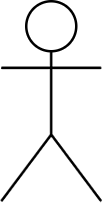
\includegraphics[scale=.1]{Capitulo3/img/actor.png} Ingresa el actor a la aplicación móvil.}
\item {
\includegraphics[scale=.05]{Capitulo3/img/proceso.png} Se muestra la vista IU Principal.}
\item {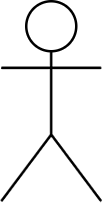
\includegraphics[scale=.1]{Capitulo3/img/actor.png} Presiona el botón de Iniciar sesión.}
\item {
\includegraphics[scale=.05]{Capitulo3/img/proceso.png} Se muestra la vista IU Inicio.}
\item {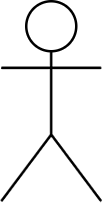
\includegraphics[scale=.1]{Capitulo3/img/actor.png} Selecciona el actor la opción de \textit{Consultar perfil}}
\item {
\includegraphics[scale=.05]{Capitulo3/img/proceso.png} Se muestra la IU Perfil}
\item {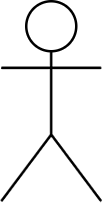
\includegraphics[scale=.1]{Capitulo3/img/actor.png} Presiona el actor el BTN Modificar documentos.}
\item {
\includegraphics[scale=.05]{Capitulo3/img/proceso.png} Se habilida la opción de IU Modificar documentos. [\textbf{\ref{cu3_2_ta_a}}]}
\item {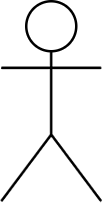
\includegraphics[scale=.1]{Capitulo3/img/actor.png} El actor ingresa la Liga electrónica del documento o lo selecciona mediante el dialogo de selección.}
  \item {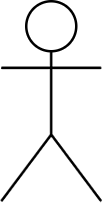
\includegraphics[scale=.1]{Capitulo3/img/actor.png} Presiona el botón para guardar sus cambios.}
  \item {
\includegraphics[scale=.05]{Capitulo3/img/proceso.png} Verifica que cumpla con la \textbf{\ref{rnl_01}}. [\textbf{\ref{cu3_2_ta_a}}]}
  \item {
\includegraphics[scale=.05]{Capitulo3/img/proceso.png} Verifica que el documento sea válido. [\textbf{\ref{cu3_2_ta_b}}] [\textbf{\ref{cu3_2_ta_c}}]}
  \item {
\includegraphics[scale=.05]{Capitulo3/img/proceso.png} Se muestra el mensaje \textbf{\ref{msjn_07}} que indica que los cambios han sido guardados.}
  \textit{Fin de caso de uso} \\  
\end{enumerate}

\textbf{\textlabel{Trayectoria alternativa A}{cu3_2_ta_a}} \\
\textbf{Condición:} El actor presiona el botón de eliminar al lado del nombre de algún documento.\\
 \begin{enumerate}[label=A\arabic*]
    \item {
\includegraphics[scale=.05]{Capitulo3/img/proceso.png} Muestra el mensaje \textbf{\ref{msjc_02}}.}
    \item {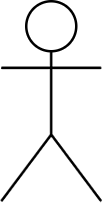
\includegraphics[scale=.1]{Capitulo3/img/actor.png} El actor confirma o cancela la operación.}
        \item {
\includegraphics[scale=.05]{Capitulo3/img/proceso.png} Muestra el mensaje \textbf{\ref{msjc_08}}, indicando que se ha borrado exitosamente el documento.}
    \item {Continua en el paso 8  de la trayectoria principal.}
    \textit{Fin de trayectoria} \\
\end{enumerate}

\textbf{\textlabel{Trayectoria alternativa A}{cu3_2_ta_a}} \\
\textbf{Condición:} El actor no proporcionó la información requerida, rompiendo la regla de negocio \textbf{\ref{rnl_01}}.\\
 \begin{enumerate}[label=A\arabic*]
    \item {
\includegraphics[scale=.05]{Capitulo3/img/proceso.png} Muestra el mensaje \textbf{\ref{msja_01}}, indicando que el actor ha dejado campos en blanco.}
    \item {Continua en el paso 9  de la trayectoria principal.} \\
    \textit{Fin de trayectoria} \\
\end{enumerate}

\textbf{\textlabel{Trayectoria alternativa B}{cu3_2_ta_b}} \\
\textbf{Condición:} El actor intento agregar un documento que no cumple con la \textbf{\ref{rnrv_10}}.\\
 \begin{enumerate}[label=B\arabic*]
    \item {
\includegraphics[scale=.05]{Capitulo3/img/proceso.png} Muestra el mensaje \textbf{\ref{msje_10}}, indicando que el documento no tiene el tamaño adecuado.}
    \item {Continua en el paso 9 de la trayectoria principal.} \\
    \textit{Fin de trayectoria} \\
\end{enumerate}

\textbf{\textlabel{Trayectoria alternativa C}{cu3_2_ta_c}} \\
\textbf{Condición:} El actor intento agregar un documento que no cumple con la \textbf{\ref{rnrv_10}}.\\
 \begin{enumerate}[label=C\arabic*]
    \item {
\includegraphics[scale=.05]{Capitulo3/img/proceso.png} Muestra el mensaje \textbf{\ref{msje_11}}, indicando que el documento tiene una liga electrónica no soportada.}
    \item {Continua en el paso 9 de la trayectoria principal.} \\
    \textit{Fin de trayectoria} \\
\end{enumerate}

\textbf{\textlabel{Trayectoria alternativa D}{cu3_2_ta_d}} \\
\textbf{Condición:} El actor selecciona la opción de \textit{Inicio} en el menú lateral MN1. \\
 \begin{enumerate}[label=D\arabic*]
    \item {
\includegraphics[scale=.05]{Capitulo3/img/proceso.png} Se redirecciona a la vista IU Inicio.} \\
    \textit{Fin de trayectoria} \\
\end{enumerate}

\textbf{\textlabel{Trayectoria alternativa E}{cu3_2_ta_e}} \\
\textbf{Condición:} El actor selecciona la opción de \textit{Perfil} en el menú lateral MN1. \\
 \begin{enumerate}[label=E\arabic*]
    \item {
\includegraphics[scale=.05]{Capitulo3/img/proceso.png} Se ejecuta el \textbf{\nameref{cu3}}.} \\
    \textit{Fin de trayectoria} \\
\end{enumerate}

\textbf{\textlabel{Trayectoria alternativa F}{cu3_2_ta_f}} \\
\textbf{Condición:} El usuario selecciona la opción de \textit{Sub-Usuarios} en el menú lateral MN1. \\
 \begin{enumerate}[label=F\arabic*]
    \item {
\includegraphics[scale=.05]{Capitulo3/img/proceso.png} Se ejecuta el \textbf{\nameref{cu4}}.} \\
    \textit{Fin de trayectoria} \\
\end{enumerate}

\textbf{\textlabel{Trayectoria alternativa G}{cu3_2_ta_g}} \\
\textbf{Condición:} El actor selecciona la opción de \textit{Alertas} en el menú lateral MN1. \\
 \begin{enumerate}[label=G\arabic*]
    \item {
\includegraphics[scale=.05]{Capitulo3/img/proceso.png} Se ejecuta el \textbf{\nameref{cu5}}.} \\
    \textit{Fin de trayectoria} \\
\end{enumerate}